\documentclass[10pt]{article}

\usepackage{amsthm}
\usepackage{amsmath}
\usepackage{amssymb}
\usepackage{mathtools}
\usepackage{graphicx}
\usepackage[colorinlistoftodos]{todonotes}
\usepackage{url}
\usepackage{xcolor}

\usepackage{pgfplots}

\usepackage[left = 1cm, top = 1cm, bottom = 2cm, right = 1cm, nohead, nofoot]{geometry}

\pgfplotsset{width=20cm, compat=1.9}

\newcommand{\C}{\mathbb{C}}  % Complex
\newcommand{\R}{\mathbb{R}}  % Real
\newcommand{\Z}{\mathbb{Z}}  % Integers
\newcommand{\N}{\mathbb{N}}  % Naturals

\newcommand{\A}{\mathbb{A}}
\newcommand{\K}{\mathbb{K}}

\title{$\A$dvanced $\C$alculus}
\author{$\C$ason $\K$onzer}
\date{October 26, 2021}



\begin{document}
\maketitle

\newpage

\section{\underline{}}
\label{sec: Problem 1}
\noindent
Represent $ f(x) = \dfrac{1}{1+x^2} $ as a Fourier cosine integral. Use Mathematica to plot the integral on the interval $[-3,3]$.
\vspace{2.5mm}
\hrule 

\vspace{7.5mm}

\begin{center}
    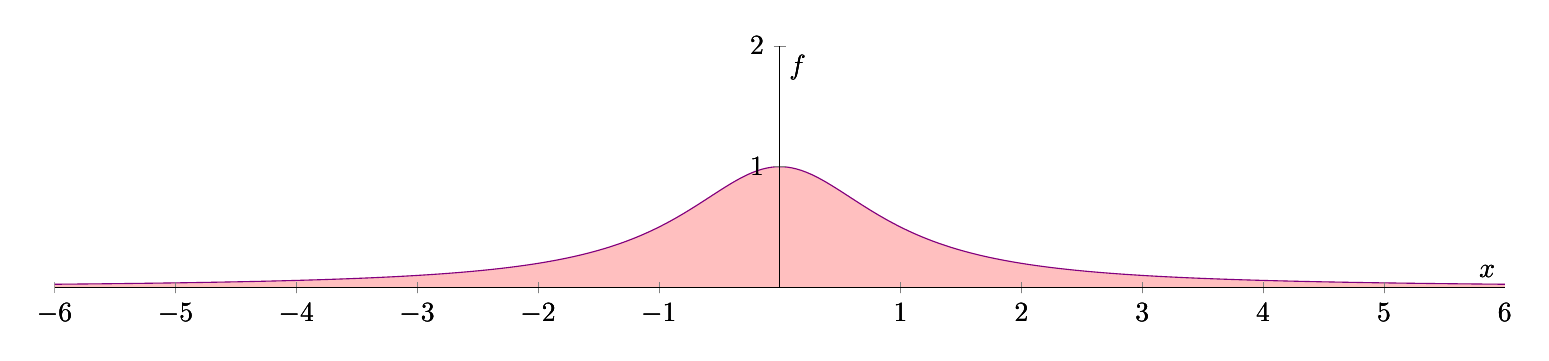
\begin{tikzpicture}
        \begin{axis}[
            xlabel = $ x $, ylabel = $ f $,
            xmin = -6, xmax = 6,
            ymin = 0, ymax = 2,
            try min ticks =  2,
            axis equal image = true,
            axis x line=center,
            axis y line=center,
            axis line style = -,
        ]
            \addplot[
                no marks,
                color = pink,
                fill
            ]
                expression[
                    domain = -10 : 10,
                    samples = 500
                ]
                    {1/(1 + x^2)}
                \closedcycle
            ;
        \end{axis}
        \begin{axis}[
            xlabel = $ x $, ylabel = $ f $,
            xmin = -6, xmax = 6,
            ymin = 0, ymax = 2,
            try min ticks =  2,
            axis equal image = true,
            axis x line=center,
            axis y line=center,
            axis line style = -,
        ]
            \addplot[
                no marks,
                color = violet
            ]
                expression[
                    domain = -10 : 10,
                    samples = 500
                ]
                    {1/(1 + x^2)}
            ;
        \end{axis}
            \begin{axis}[
                xlabel = $ x $, ylabel = $ f $,
                xmin = -6, xmax = 6,
                ymin = 0, ymax = 2,
                try min ticks =  2,
                axis equal image = true,
                axis x line=center,
                axis y line=center,
                axis line style = -,
            ]
            ;
        \end{axis}
    \end{tikzpicture} \\
\end{center}

\noindent
\textbf{Solve} the cosine integral given $ \displaystyle f(x) = \int_{0}^{\infty} A(w) \cos(wx) \,dw $, where $ \displaystyle A(w) = \frac{2}{\pi} \int_{0}^{\infty} f(v) \cos(vw) \,dv $. \\

\begin{itemize}
    \item Let $ \displaystyle \mathcal{F}_c(\gamma) = \frac{2}{\pi} \int_{0}^{\infty} \gamma(v) \cos(vw) \,dv $ and $ \displaystyle \mathcal{F}_c^{-1}(\gamma) = \int_{0}^{\infty} \gamma(w) \cos(wx) $. \\
    \item $ \displaystyle A(w) = \dfrac{2}{\pi} \int_{0}^{\infty} \dfrac{\cos(vw)}{1 + v^2} \,dv = \mathcal{F}_c(f) $. $ \dagger $ Note $ \mathcal{F}_c^{-1}(\mathcal{F}_c(\gamma)) = \gamma \dots $ \\
    \subitem From class we have, for $ x > 0 $: $ \displaystyle e^{-kx} = \dfrac{2k}{\pi} \int_{0}^{\infty} \dfrac{\cos(wx)}{k^2 + w^2} \,dw $.
    \subitem Thus, for $ v > 0 $: $ \displaystyle \alpha = e^{-v} = \dfrac{2}{\pi} \int_{0}^{\infty} \dfrac{\cos(vw)}{1 + v^2} \,dw = \mathcal{F}_c(\mathcal{F}_c^{-1}(\alpha)) $.
    \subitem $ \displaystyle A(w) = \mathcal{F}_c(f) = \mathcal{F}_c(\mathcal{F}_c^{-1}(\alpha)) = \alpha $
    \item $ \displaystyle f(x) = \mathcal{F}_c^{-1}(A) = \mathcal{F}_c^{-1}(\alpha) = \int_{0}^{\infty} e^{-w} \cos(wx) \,dw $. \\
\end{itemize}

\noindent
\textbf{Plot} the integral representations of $ f $. $ \dagger $ Use Mathematica $ \dots $ \\

\begin{center}
    \includegraphics[width=.6\textwidth]{C:/Users/cason/OneDrive - Umich/Math/Classes/Fall_2021/Advanced_Calculus/HW/WRITTEN_HW/TEX/HW4/Cosine_Plot.PNG} \\
    \includegraphics[width=\textwidth]{C:/Users/cason/OneDrive - Umich/Math/Classes/Fall_2021/Advanced_Calculus/HW/WRITTEN_HW/TEX/HW4/I_Cosine_Plot.PNG} \\
\end{center}

\newpage

\section{\underline{}}
\label{sec: Problem 2}
\noindent
Represent $ g(x) = \dfrac{x}{1+x^2} $ as a Fourier sine integral. Use Mathematica to plot the integral on the interval $[-3,3]$.
\vspace{2.5mm}
\hrule 

\vspace{7.5mm}

\begin{center}
    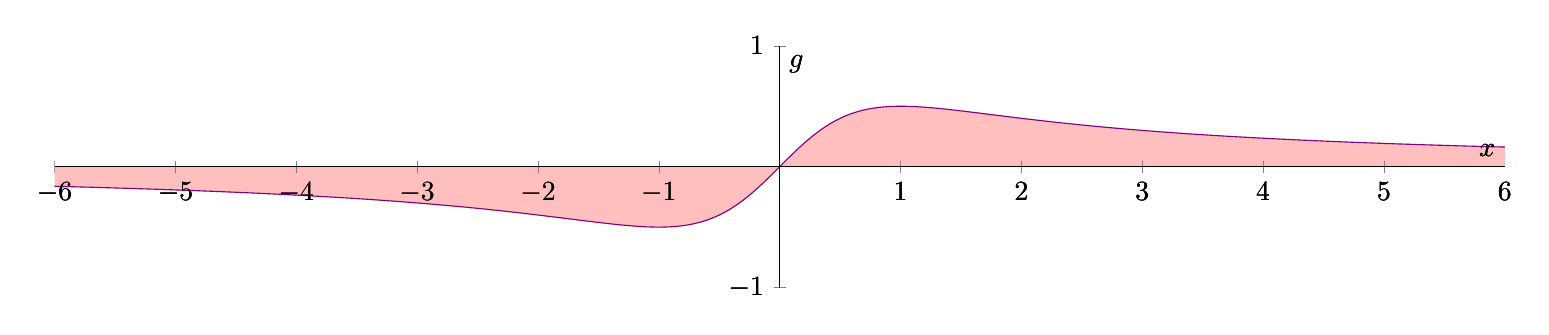
\begin{tikzpicture}
        \begin{axis}[
            xlabel = $ x $, ylabel = $ g $,
            xmin = -6, xmax = 6,
            ymin = -1, ymax = 1,
            try min ticks =  2,
            axis equal image = true,
            axis x line=center,
            axis y line=center,
            axis line style = -,
        ]
            \addplot[
                no marks,
                color = pink,
                fill
            ]
                expression[
                    domain = -10 : 10,
                    samples = 500
                ]
                    {x/(1 + x^2)}
                \closedcycle
            ;
        \end{axis}
        \begin{axis}[
            xlabel = $ x $, ylabel = $ g $,
            xmin = -6, xmax = 6,
            ymin = -1, ymax = 1,
            try min ticks =  2,
            axis equal image = true,
            axis x line=center,
            axis y line=center,
            axis line style = -,
        ]
            \addplot[
                no marks,
                color = violet
            ]
                expression[
                    domain = -10 : 10,
                    samples = 500
                ]
                    {x/(1 + x^2)}
            ;
        \end{axis}
            \begin{axis}[
                xlabel = $ x $, ylabel = $ g $,
                xmin = -6, xmax = 6,
                ymin = -1, ymax = 1,
                try min ticks =  2,
                axis equal image = true,
                axis x line=center,
                axis y line=center,
                axis line style = -,
            ]
            ;
        \end{axis}
    \end{tikzpicture} \\
\end{center}

\noindent
\textbf{Solve} the sine integral given $ \displaystyle g(x) = \int_{0}^{\infty} B(w) \sin(wx) \,dw $, where $ \displaystyle B(w) = \dfrac{2}{\pi} \int_{0}^{\infty} g(v) \sin(vw) \,dv $. \\

\begin{itemize}
    \item Let $ \displaystyle \mathcal{F}_s(\gamma) = \frac{2}{\pi} \int_{0}^{\infty} \gamma(v) \sin(vw) \,dv $ and $ \displaystyle \mathcal{F}_s^{-1}(\gamma) = \int_{0}^{\infty} \gamma(w) \sin(wx) $. \\
    \item $ \displaystyle B(w) = \dfrac{2}{\pi} \int_{0}^{\infty} \dfrac{v\sin(vw)}{1 + v^2} \,dv $. $ \dagger $ Note $ \mathcal{F}_s^{-1}(\mathcal{F}_s(\gamma)) = \gamma \dots $ 
    \subitem From class we have, for $ x > 0 $: $ \displaystyle e^{-kx} = \dfrac{2k}{\pi} \int_{0}^{\infty} \dfrac{w \sin(wx)}{k^2 + w^2} \,dw $.
    \subitem Thus, for $ v > 0 $: $ \displaystyle \beta = e^{-v} = \dfrac{2}{\pi} \int_{0}^{\infty} \dfrac{v \sin(vw)}{1 + v^2} \,dw = \mathcal{F}_s(\mathcal{F}_s^{-1}(\beta)) $.
    \subitem $ \displaystyle B(w) = \mathcal{F}_s(g) = \mathcal{F}_s(\mathcal{F}_s^{-1}(\beta)) = \beta $
    \item $ \displaystyle g(x) = \mathcal{F}_s^{-1}(B) = \mathcal{F}_s^{-1}(\beta) = \int_{0}^{\infty} e^{-w} \sin(wx) \,dw $. \\
\end{itemize}

\noindent
\textbf{Plot} the integral representations of $ g $. $ \dagger $ Use Mathematica $ \dots $ \\

\begin{center}
    \includegraphics[width=.6\textwidth]{C:/Users/cason/OneDrive - Umich/Math/Classes/Fall_2021/Advanced_Calculus/HW/WRITTEN_HW/TEX/HW4/Sine_Plot.PNG} \\
    \includegraphics[width=\textwidth]{C:/Users/cason/OneDrive - Umich/Math/Classes/Fall_2021/Advanced_Calculus/HW/WRITTEN_HW/TEX/HW4/I_Sine_Plot.PNG} \\
\end{center}

\end{document}



%%%%%%%%%%%%%%%%%%%%%%%%%%%%%%%%%%%%%%%%%%%%%%%%%%%%%%%%%%%%%%%%%%%%%%%%%%%%%%%%%%%%%%%%%%%%%%%%
%%%%%%%%%%%%%  Comments - October 26, 2021 Advanced Calculus Written Home Work #4% %%%%%%%%%%%%%